\documentclass[xcolor=dvipsnames]{beamer}

% font setup
\usepackage{libertine}
\renewcommand*\familydefault{\sfdefault}    % Linux Libertine = default sans serif
\usepackage{inconsolata}                    % Inconsolata = monospaced
\usepackage[utf8]{inputenc}
\usepackage[T1]{fontenc}
\usepackage{tikz}
\usetikzlibrary{positioning}
\usepackage[style=german]{csquotes}
\newcommand\qq{\enquote}
\newcommand\dr{\mathrm}
\usepackage[normalem]{ulem}

\usepackage{algorithm}
\usepackage{algpseudocode}
\makeatletter
\renewcommand{\ALG@name}{Algoritm}
\makeatother
\algrenewcommand\algorithmicprocedure{\textbf{procedură}}
\algrenewcommand\algorithmicend{\textbf{final}}

% Graphics and other packages
\usepackage[romanian]{babel}
\usepackage{graphicx}
\addto\captionsromanian{\renewcommand{\figurename}{Ilustrație}}
\usepackage{caption}
\usepackage{subcaption}
\usepackage[style=german]{csquotes}

% Custom macros
\newcommand{\bloc}[3]{\begin{bl}<#1->{{\large\color{Gray}{\hrulefill}}\\ \color{bleumarin}{\large \emph{#2}}}\\ \vspace*{-2mm}{\color{Gray}{\hrulefill}}\\ #3 \end{bl}} 
\newcommand{\fr}[1]{\frame{#1}}
\newcommand{\ft}[1]{\frametitle{\color{bleumarin}{\hfill #1 \hfill}}}
\newcommand{\lin}[3]{\uncover<#1->{\alert<#1>{#2}}{\vspace*{#3 ex}}}
\newcommand{\ite}[2]{\uncover<#1->{\alert<#1>{\item #2}}}
\newcommand{\vs}[1]{\vspace*{#1 ex}}
\definecolor{bleumarin}{RGB}{30,30,150} 
\definecolor{firebrick}{RGB}{178,34,34}

% Theme setup
\useoutertheme{shadow} 
\usetheme{CambridgeUS} 
\usecolortheme[named=bleumarin]{structure} 
\useoutertheme[compress]{smoothbars}

% Theme finetuning
\setbeamertemplate{items}[ball]
\setbeamertemplate{blocks}[rounded][shadow=true]
\setbeamertemplate{navigation symbols}{}
\setbeamertemplate{headline}{}  


%%%%%%%%%%%%%%%%%%%%%%%%%%%%%%%%%%%%%%%%%%%%%%%%%%%%%%%%%%%%%%%%%%%%%% 
% TITLE PAGE
\title[DREAM]{Decompilare fără \texttt{goto} cu DREAM}
\author{Adrian Manea}
\institute{510, SLA}

\date{}

\begin{document}

\maketitle

% SLIDES START HERE
%%%%%%%%%%%%%%%%%%%%%%%%%%%%%%%%%%%%%%%%%%%%%%%%%%%%%%%%%%%%%%%%%%%%%% 
\fr{
  \ft{Problema și soluția propusă}

  \lin{1}{Articolul: \textbf{No More Gotos: Decompilation Using Pattern-Independent
      Control Flow Structuring and Semantics-Preserving Transformations},
    K.\ Yakdan et al., NDSS 2015}{2}

  \lin{2}{Decompilatoarele, bazate pe analiză structurală pe baza grafului
    de control (CFG), generează instrucțiuni \texttt{goto} atunci cînd nu
    găsesc o continuare așteptată în graf.}{1}

  \lin{3}{DREAM elimină \texttt{goto} prin transformări care păstrează
    semantica și alte prelucrări logice pe graf.}{1}

  \lin{4}{Concurența: Hex-Rays și Phoenix.}{1}

  \lin{5}{Benchmark: GNU \texttt{coreutils}.}{1}
}

\fr{
  \ft{Procedura de ansamblu}

  \lin{1}{Eliminarea \texttt{goto} se va putea face ținînd cont că:}{0}
  \begin{itemize}
    \ite{2}{Structurile de control din program au un singur punct de intrare
      și un singur punct succesor $ \Rightarrow $ se pot simplifica;}
    \ite{3}{Tipul și posibilele ramificații ale structurilor de control se pot
      analiza folosind \emph{logică} pe CFG.}
  \end{itemize}

  \lin{4}{Etape, în mare:}{0}
  \begin{enumerate}
    \ite{5}{Se alcătuiește CFG;}
    \ite{6}{Se structurează CFG folosind și transformări invariante semantic;}
    \ite{7}{Se obține AST (arborele de sintaxă abstractă);}
    \ite{8}{Se fac optimizări post-structurare (redenumiri de variabile, evidențierea
      funcțiilor pe șiruri de caractere, simplificarea ramificațiilor).}
  \end{enumerate}
}

\fr{
  \ft{Etapele DREAM}

  \begin{enumerate}
    \ite{1}{\emph{Dezasamblează} binarul folosind IDA Pro $ \Rightarrow $ CFG;}
    \ite{2}{\emph{Analiza fluxului de date}, inclusiv propagarea constantelor și
      eliminarea codului mort (inaccesibil);}
    \ite{3}{\emph{Inferă tipurile variabilelor}, folosind TIE;}
    \ite{4}{\textbf{\underline{Structurează CFG}}:}
    \begin{itemize}
      \ite{5}{\textbf{Nu folosește pattern matching} (``pattern independent'');}
      \ite{6}{Folosește DFS (depth-first search);}
      \ite{7}{Tratează separat zonele cu cicluri de cele fără cicluri;}
      \ite{8}{Aplică transformări care păstrează semantica;}
      \ite{9}{Aplică optimizări finale.}
    \end{itemize}
  \end{enumerate}
}

\fr{
  \ft{Transferul controlului (\emph{Reaching Condition})}

  \lin{1}{Fie $ G(N, E, n_{in}) $ graful de control.}{0}

  \lin{2}{Cu DFS între $ n_{\text{src}} $ și $ n_{\text{exit}} $ fixate obținem un
    subgraf aciclic $ S_G(n_s, n_e) $ (``slice'') și drumurile \emph{simple} între
    $ n_s $ și $ n_e $ (similar: Cifuentes).}{0}

  \lin{3}{
    \begin{center}
      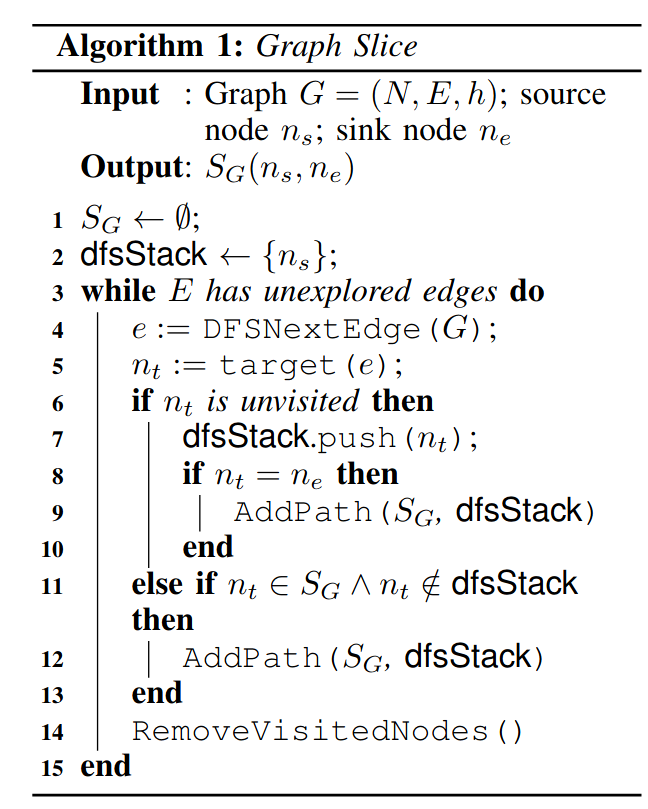
\includegraphics[scale=0.22]{img/slice-alg.png}
    \end{center}
  }{4}
}

\fr{
  \ft{Exemplu}

  \lin{1}{
    \begin{figure}
      \centering
      \begin{subfigure}[t]{0.67\textwidth}
        \centering
        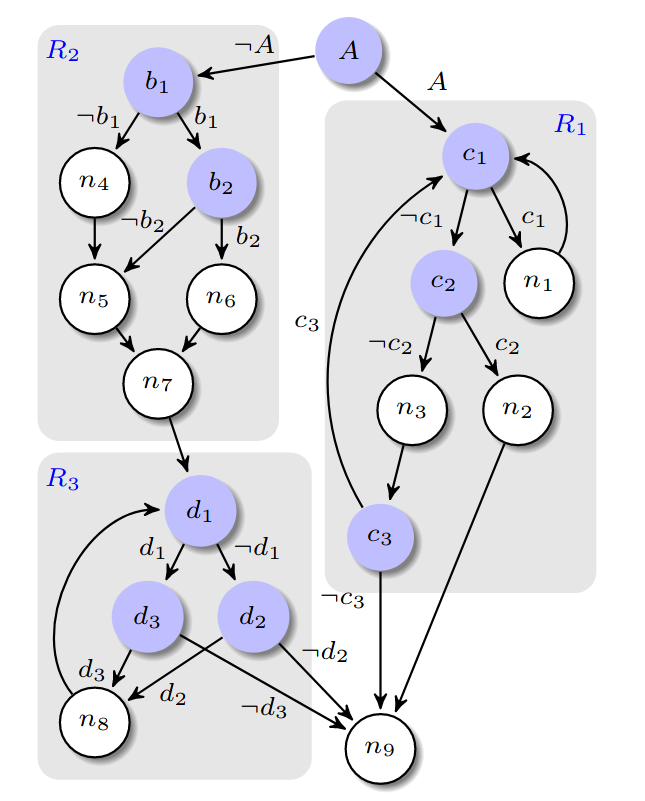
\includegraphics[scale=0.24]{img/cfg.png}
        \caption{CFG -- exemplu de lucru}
      \end{subfigure}
      ~
      \begin{subfigure}[t]{0.2\textwidth}
        \centering
        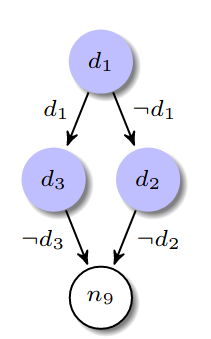
\includegraphics[scale=0.3]{img/slice-ex.png}
        \caption{$ S_G(d_1, n_9) $}
      \end{subfigure}
    \end{figure}}{0}

  \lin{2}{\hfill$ d_1 \to n_9 \Leftrightarrow (d_1 \land \neg d_3) \lor (\neg d_1 \land \neg d_2) $}{0}
}

\fr{
  \ft{Structurarea zonelor aciclice}

  \lin{1}{Ideea: Putem ordona un graf orientat aciclic inversînd ordinea
    parcurgerii DF (ordine topologică);}{2}

  \lin{2}{Calculăm condiția de accesibilitate de la intrare la fiecare nod;}{1}

  \lin{3}{Obținem un AST al nodurilor în ordine topologică, \emph{ne-optim};}{1}

  \lin{4}{Rafinăm acest AST folosind logică (condiții complementare, \texttt{switch} pentru
    clustere de control) și eventuale \texttt{if-then-else} în cascadă.}{1}

  \lin{5}{Exemplu: În regiunea $ R_2 $, avem \emph{condițiile complementare}
    \[
      \texttt{if (b1 AND b2) then n6} \text{ și } \texttt{if (\~ b1 OR \~b2) then n4 or n5}.
    \]}{0}

  \lin{6}{Putem structura sub forma \texttt{if (b1 AND b2) then n6 else n5}.}{0}
}

\fr{
  \ft{Structurarea zonelor cu cicluri}

  \begin{enumerate}
    \ite{1}{Găsim nodurile care conduc la bucle;}
    \ite{2}{Refacem zonele ciclice $ \Rightarrow $ o singură intrare, un singur succesor;}
    \ite{3}{Obținem AST pentru buclă;}
    \ite{4}{Determinăm tipul buclei și condiția de intrare prin analiza AST;}
  \end{enumerate}

  \lin{5}{\begin{center} 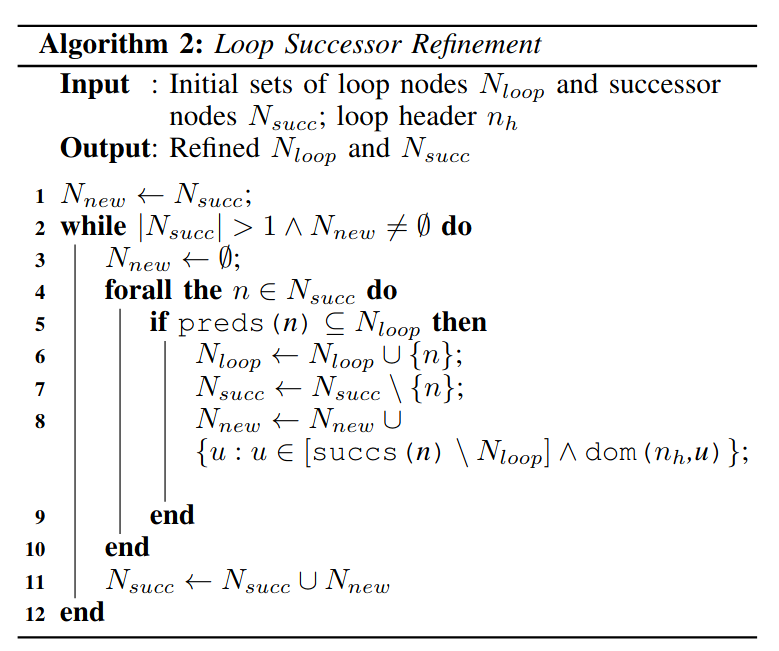
\includegraphics[scale=0.25]{img/loop-ref.png} \end{center}}{0}
}

\fr{
  \ft{Identificarea logică a buclelor}


  \lin{1}{
    \begin{center}
      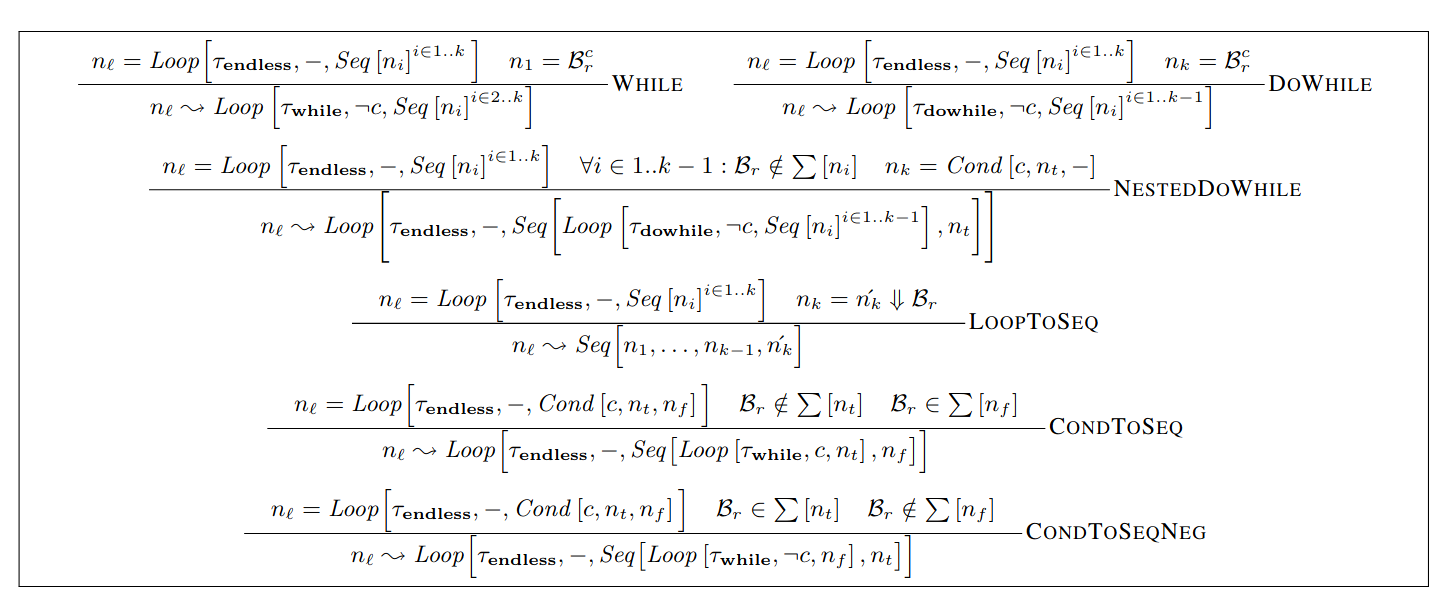
\includegraphics[scale=0.24]{img/loop-type.png}
    \end{center}
  }{0}

  \lin{2}{+ Transformări care \emph{păstrează semantica} buclei prin înregistrarea
    punctelor de intrare.}{0}
}

\fr{
  \ft{Optimizări finale (pentru lizibilitate)}

  \begin{itemize}
    \ite{1}{Simplificarea structurilor de control:}
    \begin{itemize}
      \ite{2}{\texttt{if (c) then (x = v) else (x = w)} $ \leadsto $
        \texttt{x = c ? v : w};}
      \ite{3}{Se transformă \texttt{while} în \texttt{for} oricît de des este posibil;}
    \end{itemize}
    \ite{4}{Identificarea funcțiilor pe șiruri de caractere:}
    \begin{itemize}
      \ite{5}{\texttt{strcpy, strlen, strcmp} sînt înlocuite de definițiile lor de compilator,
        așa că DREAM le evită sau le evidențiază în mod special;}
    \end{itemize}
    \ite{6}{Redenumirea variabilelor, e.g.\ cele corespunzătoare API-urilor folosite.}
  \end{itemize}
}

\fr{
  \ft{Teste și comparații}

  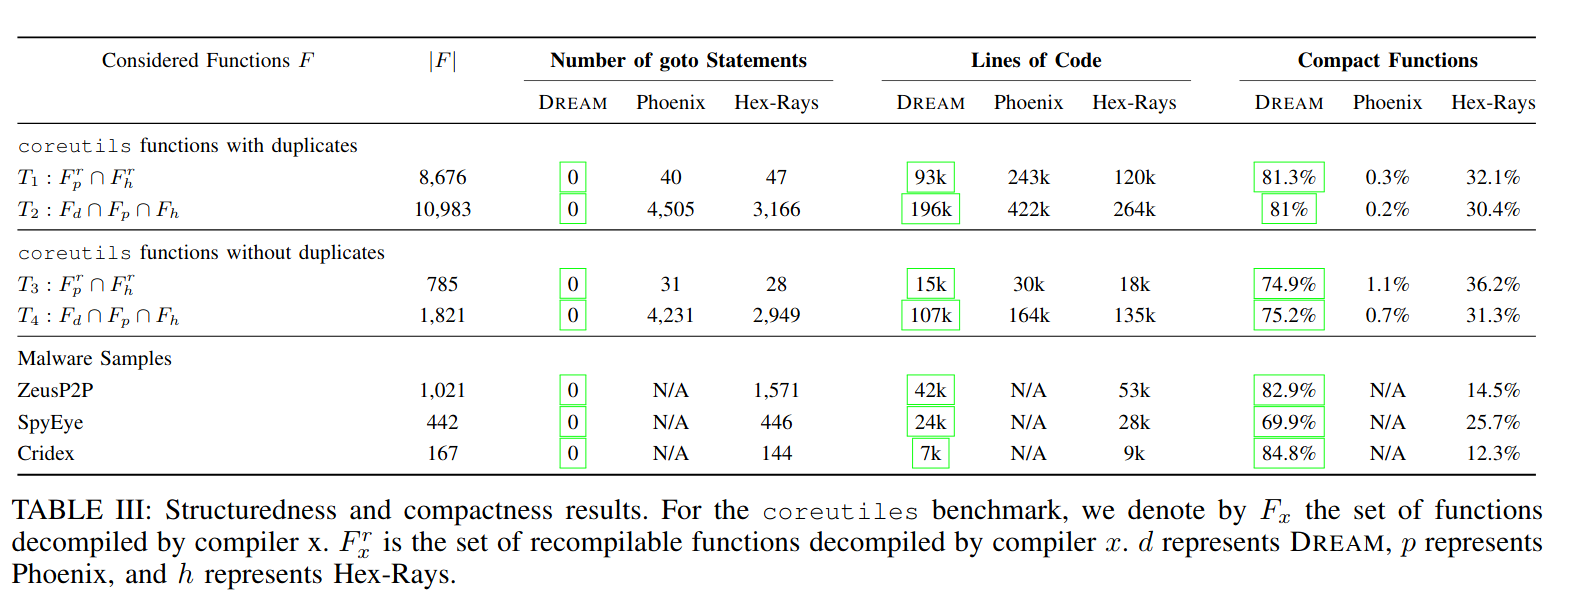
\includegraphics[scale=0.22]{img/results.png}

}
%%%%%%%%%%%%%%%%%%%%%%%%%%%%%%%%%%%%%%%%%%%%%%%%%%%%%%%%%%%%%%%%%%%%%% 

% % Bibliography
% \begin{frame}[allowframebreaks]
%   \ft{Bibliografie și lecturi suplimentare}
%   \bibliography{../tex/semdis.bib}
%   \bibliographystyle{apalike}
%   \nocite{*}
% \end{frame}

\end{document}

